\documentclass[11pt,a4paper]{report}
\usepackage[utf8]{inputenc}
\usepackage{amsmath}
\usepackage{amsfonts}
\usepackage{amssymb}
\usepackage{fancyhdr}
\usepackage{enumitem}
\usepackage[dvipsnames]{xcolor}
\usepackage{graphicx}
\usepackage{caption}
\usepackage{hyperref}
\usepackage{helvet}
\usepackage{titlesec}
\usepackage{stmaryrd}
\usepackage{array}
\usepackage{setspace}
\usepackage{stmaryrd}
\usepackage{bbold}
\usepackage{listings}
\usepackage{xcolor}

\DeclareMathOperator*{\argmax}{arg\,max}

\definecolor{codegreen}{rgb}{0,0.6,0}
\definecolor{codegray}{rgb}{0.5,0.5,0.5}
\definecolor{codepurple}{rgb}{0.58,0,0.82}
\definecolor{backcolour}{rgb}{0.95,0.95,0.92}

\lstdefinestyle{mystyle}{
    backgroundcolor=\color{backcolour},   
    commentstyle=\color{codegreen},
    keywordstyle=\color{magenta},
    numberstyle=\tiny\color{codegray},
    stringstyle=\color{codepurple},
    basicstyle=\ttfamily\footnotesize,
    breakatwhitespace=false,         
    breaklines=true,                 
    captionpos=b,                    
    keepspaces=true,                 
    numbers=left,                    
    numbersep=5pt,                  
    showspaces=false,                
    showstringspaces=false,
    showtabs=false,                  
    tabsize=2
}
\lstset{style=mystyle}

\usepackage{tikz}
\usepackage{xparse}
\usepackage{tikz}
\usetikzlibrary{matrix,backgrounds}
\pgfdeclarelayer{myback}
\pgfsetlayers{myback,background,main}

\tikzset{mycolor/.style = {line width=1bp,color=#1}}%
\tikzset{myfillcolor/.style = {draw,fill=#1}}%

\NewDocumentCommand{\highlight}{O{blue!40} m m}{%
\draw[mycolor=#1] (#2.north west)rectangle (#3.south east);
}

\NewDocumentCommand{\fhighlight}{O{blue!40} m m}{%
\draw[myfillcolor=#1] (#2.north west)rectangle (#3.south east);
}



\titleformat{\section}{\huge\center\bfseries\fontsize{20}{20}}{}{1em}{}
\titlespacing*{\section}{0pt}{*0}{3em}
  
\renewcommand{\familydefault}{\sfdefault}
\renewcommand*\contentsname{Table of contents}
\renewcommand\thesection{\Roman{section}}
\renewcommand\thesubsection{\arabic{subsection}}

\title{
\textbf{\huge AI Project}\leavevmode \\
}
\author{\Large Robin MENEUST}

\date{\Large August 2023}
%\maketitle
\makeatletter

\begin{document}

\onehalfspacing
\begin{titlepage}
\vspace*{\stretch{1}}
\hrulefill
\begin{center}
    \@title
\end{center}
\hrulefill
\vspace*{2cm}
\begin{center}
	\@author
\end{center}

\vspace*{\stretch{2}}
\begin{center}
       \Large \@date
\end{center}   
\end{titlepage}
\makeatother


\tableofcontents

\newpage

\noindent

\section{Introduction}

\subsection{Softmax derivative}

Softmax :
\begin{equation}
    s_{z_i}(z_1, z_2, ... z_n) = \frac{e^{z_i}}{\sum\limits_{j=1}^{n} e^{z_j}}
\end{equation}
Derivative :

\begin{equation}
\begin{split}
    \frac{\partial s_{z_i}}{\partial z_i} &= \frac{\partial \left(\frac{e^{z_i}}{\sum\limits_{j=1}^{n} e^{z_j}}\right)}{\partial z_i}\\
    &= \frac{\partial \left(\frac{e^{z_i}}{k + e^{z_i}}\right)}{\partial z_i},\ \ \text{ where } k = \sum\limits_{j=1,\ j\neq i}^n e^{z_j}\\
    &= \frac{\partial\left( 1-\frac{k}{k+e^{z_i}}\right)}{\partial z_i}\\
    &= \frac{ke^{z_i}}{(k+e^{z_i})^2}\\
    &= \left(\sum\limits_{j=1,\ j\neq i}^{n} e^{z_j}\right)\frac{e^{z_i}}{\left(\left(\sum\limits_{j=1,\ j\neq i}^{n} e^{z_j}\right)+e^{z_i}\right)^2}\\
    &= \left(\sum\limits_{j=1,\ j\neq i}^{n} e^{z_j}\right)\frac{e^{z_i}}{\left(\sum\limits_{j=1}^{n} e^{z_j}\right)^2}\\
    &= \left(\left(\sum\limits_{j=1}^{n} e^{z_j}\right)-e^{z_i}\right)\frac{e^{z_i}}{\left(\sum\limits_{j=1}^{n} e^{z_j}\right)^2}\\
    &= e^{z_i}\left(\frac{1}{\sum\limits_{j=1}^{n} e^{z_j}} - 
    \frac{s_{z_i}^2}{e^{z_i}}\right)\\
    &= s_{z_i} - s_{z_i}^2\\
    &= s_{z_i} (1 - s_{z_i})\\
\end{split}
\end{equation}\\

And:
\begin{equation}
\begin{split}
    \frac{\partial s_{z_{k}}}{\partial z_{k\neq i}}  &= \frac{\partial \left(\frac{e^{z_i}}{\sum\limits_{j=1}^{n} e^{z_j}}\right)}{\partial z_{k\neq i}}\\
    &= e^{z_i}\frac{\partial \left(\frac{1}{c + e^{z_{k}}}\right)}{\partial z_{k\neq i}},\ \ \text{ where } c = \sum\limits_{j=1,\ j\neq k}^n e^{z_j}\\
    &= -e^{z_i}\frac{e^{z_k}}{(c+e^{z_{k}})^2}\\
    &= -\frac{e^{z_i}e^{z_k}}{\left(\left(\sum\limits_{j=1,\ j\neq k}^n e^{z_j}\right)+e^{z_{k}}\right)^2}\\
    &= -\frac{e^{z_i}e^{z_k}}{\left(\sum\limits_{j=1}^n e^{z_j}\right)^2}\\
    & - s_{z_i}s_{z_k}
\end{split}
\end{equation}

So we have :

\begin{equation}
\begin{split}
\frac{\partial s_{z_k}}{\partial z_{i}} &= 
    \begin{cases}
       s_{z_i} (1 - s_{z_i}) &\text{ if } i=k\\
       -s_{z_i} s_{z_k} &\text{ else } \\
    \end{cases}\\
    &= s_{z_i}\left( \delta_{ik} - s_{z_k}\right)
\end{split}
\end{equation}

And
\begin{equation}
\begin{split}
    \frac{\partial E_i}{\partial z_k^{(n-1)}} &= \frac{\partial E_i}{\partial s_{z_i}} \frac{\partial s_{z_i}}{\partial z_k^{(n-1)}}\\
    &= \left( s_{z_i} - \hat{y_i}\right) s_{z_i}\left( \delta_{ik} - s_{z_k} \right)
\end{split}
\end{equation}

\subsection{Definitions and standard functions derivatives}

Let :
\begin{enumerate}
    \item $C$ be the total cost function
    \item $y_i$ be the output (prediction) $i$
    \item $\hat{y_i}$ be the expected output $i$
    \item $C_i$ be the cost for output $i$ (e.g. $\frac{1}{2}\left(\hat{y_i}-y_i\right)^2$
    \item $w_{i,j}^{(l)}$ be the weight of the neuron $j$ of the layer $l-1$ for the neuron $i$ of the layer $l$
    \item $z_i^{(l)}$ be the weighted sum for the neuron $i$ of the layer $l$ (activation function input)
    \item $a_i^{(l)} = g^{(l)}(z_i^{(l)})$ be the output of the neuron $i$ of the layer $l$ (activation function output)
    \item $b_i^{(l)}$ be the bias of the neuron $i$ of the layer $l$
    \item $L$ be the number of layers and the index of the output layer (layers index goes from $1$ to $L$)
    \item $n_l$ be the number of neurons in the layer $l$
    \item The derivative of Sigmoid $\sigma$ is $\sigma (1-\sigma)$
    \item The derivative of Softmax $s_{z_i}(z_i)$ is $s_{z_i}(z_i)\left( 1 - s_{z_i}(z_i)\right)$
\end{enumerate}

\newpage
\section{Back-propagation}

\subsection{Output layer L}

Here we consider that the activation function of the layer $L$ is Softmax $s$.


\begin{equation*}
    \frac{\partial C}{\partial w_{i,j}^{(L)}} = \frac{\partial C}{\partial a_i^{(L)}} \frac{\partial a_i^{(L)}}{\partial z_i^{(L)}} \frac{\partial z_i^{(L)}}{\partial w_{i,j}^{(L)}}
\end{equation*}

Where

\begin{equation*}
    \frac{\partial C}{\partial a_i^{(L)}} = \frac{\partial \frac{1}{n_{l}} \sum\limits_{k=1}^{n_{L}} C_k}{\partial a_i^{(L)}} = \frac{1}{n_{L}} \sum\limits_{k=1}^{n_{l}} \frac{\partial C_k}{\partial a_i^{(L)}} = \frac{1}{n_{L}}\frac{\partial C_i}{\partial a_i^{(L)}}
\end{equation*}

\begin{equation*}
    \frac{\partial a_i^{(L)}}{\partial z_i^{(L)}} = \frac{\partial s_{z_i^{(L)}}}{\partial z_i^{(L)}} = g'^{(L)}(z_i^{(L)})
\end{equation*}

\begin{equation*}
    \frac{\partial z_i^{(L)}}{\partial w_{i,j}^{(L)}} = \frac{\partial \left( \sum\limits_{k=1}^{n_{L-1}} \left(w_{i,k}^{(L)} a_i^{(L-1)}\right) + b_i^{(L)}\right)}{\partial w_{i,j}^{(L)}} = \sum\limits_{k=1}^{n_{L-1}}\left( \frac{\partial w_{i,k}^{(L)} a_i^{(L-1)}}{\partial w_{i,j}^{(L)}}\right) + \frac{\partial b_i^{(L)}}{\partial w_{i,j}^{(L)}} = a_j^{(L-1)}
\end{equation*}

For the bias it's almost the same equation:

\begin{equation*}
    \frac{\partial C}{\partial b_i^{(L)}} = \frac{\partial C}{\partial a_i^{(L)}} \frac{\partial a_i^{(L)}}{\partial z_i^{(L)}} \frac{\partial z_i^{(L)}}{\partial b_i^{(L)}}
\end{equation*}

Where

\begin{equation*}
    \frac{\partial z_i^{(L)}}{\partial b_i^{(L)}} = \frac{\partial \left( \left(\sum\limits_{k=1}^{n_{L-1}} w_{i,k}^{(L)} a_i^{(L-1)}\right) + b_i^{(L)}\right)}{\partial b_i^{(L)}} = \sum\limits_{k=1}^{n_{L-1}}\left( \frac{\partial w_{i,k}^{(L)} a_i^{(L-1)}}{\partial b_i^{(L)}}\right) + \frac{\partial b_i^{(L)}}{\partial b_i^{(L)}} = 1 
\end{equation*}

\subsection{Layer L-1}


Here we consider that the activation function of the layer $L-1$ and the other ones except L is sigmoid $\sigma$.


\begin{equation*}
    \frac{\partial C}{\partial w_{i,j}^{(L-1)}} = \frac{\partial C}{\partial a_i^{(L-1)}} \frac{\partial a_i^{(L-1)}}{\partial z_i^{(L-1)}} \frac{\partial z_i^{(L-1)}}{\partial w_{i,j}^{(L-1)}}
\end{equation*}

Where

\begin{equation*}
    \frac{\partial a_i^{(L-1)}}{\partial z_i^{(L-1)}} = \frac{\partial \sigma}{\partial z_i^{(L-1)}} = g'^{(L-1)}(z_i^{(L-1)})
\end{equation*}

\begin{equation*}
    \frac{\partial z_i^{(L-1)}}{\partial w_{i,j}^{(L-1)}} = \frac{\partial \left( \sum\limits_{k=1}^{n_{L-2}} \left(w_{i,k}^{(L-1)} a_i^{(L-2)}\right) + b_i^{(L-1)}\right)}{\partial w_{i,j}^{(L-1)}} = \sum\limits_{k=1}^{n_{L-2}}\left( \frac{\partial w_{i,k}^{(L-1)} a_i^{(L-2)}}{\partial w_{i,j}^{(L-1)}}\right) + \frac{\partial b_i^{(L-1)}}{\partial w_{i,j}^{(L-1)}} = a_j^{(L-2)}
\end{equation*}



\begin{equation*}
    \frac{\partial C}{\partial a_i^{(L-1)}} = \sum\limits_{k=1}^{n_{L}}\frac{\partial C}{\partial a_k^{(L)}} \frac{\partial a_k^{(L)}}{\partial z_k^{(L)}} \frac{\partial z_k^{(L)}}{\partial a_i^{(L-1)}}
\end{equation*}

We already calculated the 2 first derivatives in the previous subsection, and for the last one:

\begin{equation*}
    \frac{\partial z_k^{(L)}}{\partial a_i^{(L-1)}} = \frac{\partial \left( \sum\limits_{p=1}^{n_{L-1}} \left(w_{k,p}^{(L)} a_k^{(L-1)}\right) + b_k^{(L)}\right)}{\partial a_i^{(L-1)}} = \sum\limits_{p=1}^{n_{L-1}}\left( \frac{\partial w_{k,p}^{(L)} a_k^{(L-1)}}{\partial a_i^{(L-1)}}\right) + \frac{\partial b_k^{(L)}}{\partial a_i^{(L-1)}} = w_{k,i}^{(L)}
\end{equation*}

\subsection{Layer $l<L$}

\begin{equation*}
    \frac{\partial C}{\partial w_{i,j}^{(l)}} = \frac{\partial C}{\partial a_i^{(l)}} \frac{\partial a_i^{(l)}}{\partial z_i^{(l)}} \frac{\partial z_i^{(l)}}{\partial w_{i,j}^{(l)}} = \frac{\partial C}{\partial a_i^{(l)}} g'^{(l)}(z_i^{(l)}) a_j^{(l-1)}
\end{equation*}

Where if $l<L$:

\begin{equation*}
    \frac{\partial C}{\partial a_i^{(l)}} = \sum\limits_{k=1}^{n_{l+1}}\frac{\partial C}{\partial a_k^{(l+1)}} \frac{\partial a_k^{(l+1)}}{\partial z_k^{(l+1)}} \frac{\partial z_k^{(l+1)}}{\partial a_i^{(l)}} = \sum\limits_{k=1}^{n_{l+1}}\frac{\partial C}{\partial a_k^{(l+1)}}g'^{(l+1)}(z_k^{(l+1)}) w_{k,i}^{(l+1)}
\end{equation*}

Otherwise if $l=L$:

\begin{equation*}
\begin{split}
    \frac{\partial C}{\partial a_i^{(L)}} &= \frac{1}{n_{L}}\frac{\partial C_i}{\partial a_i^{(L)}}
\end{split}
\end{equation*}

\subsection{Algorithm}

\textbf{Note}: This algorithm is not optimized, we should use the fact that we are using matrices.

\subsubsection{Step 1: feed-forward and store values}

\begin{lstlisting}[language=Python]
# input: input vector, fed to this network
# getWeightedSum(layerIndex, prevLayerValues) (z_i)
# activationFunction(layerIndex, input) (a_i)

outputs = []
weightedSums = []

outputs[0] = getWeightedSum(0, input)
weightedSums[0] = activationFunction(i, outputs[0])

for(i in range(len(layers)):
    weightedSums[i] = getWeightedSum(i, outputs[i-1])
    outputs[i] = activationFunction(i, weightedSums[i])
\end{lstlisting}

\newpage
\subsubsection{Step 2: Back-propagation}
\begin{lstlisting}[language=Python]
# dC/da_k * da_k/dz_k
currentCostDerivatives = getCostDerivatives(outputs[len(layers)-1], expectedOutput) # vector of dC/da_k for all k
activationDerivatives = getActivationDerivatives(len(layers)-1, weightedSums[getNbLayers()-1]); # vector of da_k/dz_k for all k

for(i in range(getLayerSize(len(layers) - 1)):
    currentCostDerivatives[i] *= (1.0f/getLayerSize(len(layers) - 1) * activationDerivatives[i];


for(l in range(len(layers)-1,-1,-1):
    # Next cost derivatives computation
    if l>0:
        nextCostDerivatives = []
        for(i in range(getLayerSize(l-1))):
            nextCostDerivatives[i] = 0
            for(k in range(getLayerSize(l))):
                nextCostDerivatives[i] += currentCostDerivatives[k] * getWeight(l,k,i) # dC/da_k * da_k/dz_k * dz_k/da_i

    # Adjust the weights and biases of the current layer

    prevLayerOutput = outputs[l-1] if l>0 else input
    
    for(i in range(getLayerSize(l))):
        for(j in range(len(prevLayerOutput)):
            setWeight(l,i,j) -= lr * currentCostDerivatives[i] * prevLayerOutput[j] # lr = learning rate and we have dC/da_k * da_k/dz_k * dz_k/dw_i,j
            setBias(l,i) -= lr * currentCostDerivatives[i] # dC/da_k * da_k/dz_k

    currentCostDerivatives = nextCostDerivatives
   
\end{lstlisting}

\newpage
\subsection{Improvement: mini-batch}

Instead of training only once all the examples one by one, we will randomly create batches of examples. So for all epoch and for all batch in the epoch, we feed-forward all the examples of the batch and we calculate the error for each. Then we modify the previous algorithm to propagate all the batch derivatives vector and when we adjust a parameter we use the mean derivative of all the batch derivatives.
We will now send several examples (of the same batch) to our function for thee back-propagation (batch with several inputs instead of one input).\\
Here we will choose to only train on complete batches, so if there are leftovers after grouping items in batch of the same size, we won't use them.

\subsubsection{Step 1: feed-forward and store values}

\begin{lstlisting}[language=Python]
# batch: list of inputs vector, fed to this network
# getWeightedSum(layerIndex, prevLayerValues, batchSize) (list of vectors z_i of the layer layerIndex of all items in the batch: it's a matrix)
# activationFunction(layerIndex, input) (list of vectors a_i of the layer layerIndex of all items in the batch: it's a matrix)

outputs = []
weightedSums = []

outputs[0] = getWeightedSum(0, batch, len(batch))
weightedSums[0] = activationFunction(i, outputs[0], len(batch))

for(i in range(len(layers)):
    weightedSums[i] = getWeightedSum(i, outputs[i-1], len(batch))
    outputs[i] = activationFunction(i, weightedSums[i], len(batch))
\end{lstlisting}

\newpage
\subsubsection{Step 2: Back-propagation}
\begin{lstlisting}[language=Python]
# dC/da_k * da_k/dz_k
currentCostDerivatives = getCostDerivatives(outputs[len(layers)-1], expectedOutput, len(batch)) # Matrix of dC/da_k for all batch item and for all k
activationDerivatives = getActivationDerivatives(len(layers)-1, weightedSums[getNbLayers()-1], len(batch)) # Matrix of da_k/dz_k for all batch item and for all k


for(b in range(len(batch))):
    for(i in range(getLayerSize(len(layers) - 1)):
        currentCostDerivatives[b][i] *= (1.0f/getLayerSize(len(layers) - 1) * activationDerivatives[b][i];


for(l in range(len(layers)-1,-1,-1):
    # Next cost derivatives computation
    if l>0:
        nextCostDerivatives = []
        for(b in range(len(batch))):
            nextCostDerivatives[b] = []
            for(i in range(getLayerSize(l-1))):
                nextCostDerivatives[b][i] = 0
                for(k in range(getLayerSize(l))):
                    nextCostDerivatives[b][i] += currentCostDerivatives[b][k] * getWeight(l,k,i) # dC/da_k * da_k/dz_k * dz_k/da_i

    # Adjust the weights and biases of the current layer

    prevLayerOutput = outputs[l-1] if l>0 else batch
    
    for(i in range(getLayerSize(l))):
        for(j in range(len(prevLayerOutput)):
            # Mean of the derivatives
            deltaWeight = 0
            deltaBias = 0
            for(b in range(len(batch))):
                deltaWeight += currentCostDerivatives[b][i] * prevLayerOutput[b][j]
                deltaBias += currentCostDerivatives[b][i]
            deltaWeight /= len(batch)
            deltaBias /= len(batch)

            # Adjust the parameters
            setWeight(l,i,j) -= lr * deltaWeight # lr = learning rate and we have dC/da_k * da_k/dz_k * dz_k/dw_i,j
            setBias(l,i) -= lr * deltaBias # dC/da_k * da_k/dz_k

    currentCostDerivatives = nextCostDerivatives
   
\end{lstlisting}

\newpage
\section{Conv2D, Max-pooling and flatten layers}

\subsection{Conv2D Layer}
Here we will look at the following example :
\begin{enumerate}
    \item Input: 3x3 matrix $w_I = 3$
    \item Filter: 2x2 matrix $w_F = 2$
    \item Number of output matrices: 3
    \item Padding $p$ (Number of lines and columns of zeros added). We want in this example to get an output with the same dimensions as the input. Additionally, if the input matrix length and width are equal we need $w_I + p - w_F + 1$ iterations to read a full row, this number will be output matrix width. Hence we have: $w_I + p - w_F + 1 = w_I \Leftrightarrow p = w_F - 1$. Here $p = 1$
    \item Activation function = ReLU : We use it to keep positive values for the next layers
\end{enumerate}
\subsubsection{Feed-forward}

For each filter $Fn$ :

\begin{equation}
Fn = \begin{pmatrix}
Fn_{1,1} & Fn_{1,2} \\
Fn_{2,1} & Fn_{2,2} \\
\end{pmatrix}
\end{equation}

\begin{equation}
input = I = \begin{pmatrix}
I_{1,1} & I_{1,2} & I_{1,3} \\
I_{2,1} & I_{2,2} & I_{2,3} \\
I_{3,1} & I_{3,2} & I_{3,3} \\
\end{pmatrix}
\end{equation}

We add padding, if $p$ is odd then we add more one more row and column of zero on the last row and column, otherwise there is the same padding on every sides. In this example $p = 1$ is odd and $p/2 = 0$, thus we don't add zeros on the upper and left sides (because $p/2 = 0$), but we add one row and one columns on the lower and right sides.

\begin{equation}
input = I_{pad} = \begin{pmatrix}
I_{1,1} & I_{1,2} & I_{1,3} & 0 \\
I_{2,1} & I_{2,2} & I_{2,3} & 0 \\
I_{3,1} & I_{3,2} & I_{3,3} & 0 \\
0       & 0       & 0       & 0 \\
\end{pmatrix}
\end{equation}


\begin{equation}
output = On = Conv\left(
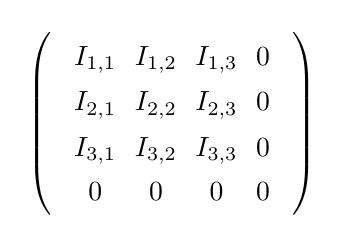
\begin{tikzpicture}[baseline=-\the\dimexpr\fontdimen22\textfont2\relax ]
\matrix (m)[matrix of math nodes,left delimiter=(,right delimiter=)]
{
I_{1,1} & I_{1,2} & I_{1,3} & 0 \\
I_{2,1} & I_{2,2} & I_{2,3} & 0 \\
I_{3,1} & I_{3,2} & I_{3,3} & 0 \\
0       & 0       & 0       & 0 \\
};

\begin{pgfonlayer}{myback}
\fhighlight[green!30]{m-2-1}{m-3-2}
\end{pgfonlayer}
\end{tikzpicture},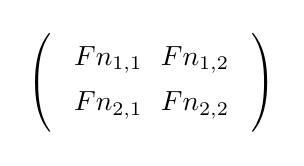
\begin{tikzpicture}[baseline=-\the\dimexpr\fontdimen22\textfont2\relax ]
\matrix (m)[matrix of math nodes,left delimiter=(,right delimiter=)]
{
Fn_{1,1} & Fn_{1,2} \\
Fn_{2,1} & Fn_{2,2} \\
};

\begin{pgfonlayer}{myback}
\fhighlight[green!30]{m-1-1}{m-2-2}
\end{pgfonlayer}
\end{tikzpicture}
\right)
\end{equation}

\begin{equation*}
=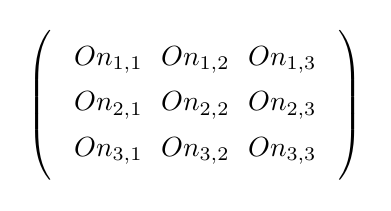
\begin{tikzpicture}[baseline=-\the\dimexpr\fontdimen22\textfont2\relax ]
\matrix (m)[matrix of math nodes,left delimiter=(,right delimiter=)]
{
On_{1,1} & On_{1,2} & On_{1,3} \\
On_{2,1} & On_{2,2} & On_{2,3} \\
On_{3,1} & On_{3,2} & On_{3,3} \\
};

\begin{pgfonlayer}{myback}
\fhighlight[green!30]{m-2-1}{m-2-1}
\end{pgfonlayer}
\end{tikzpicture}
\end{equation*}

Here, for instance, $On_{2,1} = ReLU(I_{2,1} \times Fn_{1,1} + I_{2,2} \times Fn_{1,2} + I_{3,1} \times Fn_{2,1} + I_{3,2} \times Fn_{2,2}$)


\subsubsection{Back-propagation}

We need to calculate two derivatives for each input matrices :

\begin{enumerate}
    \item One to continue the back-propagation in the previous layers
    \item Another one to adjust the filters values (similarly to the weights of the Dense layers)
\end{enumerate}

Let's begin with the first one: 

\begin{equation}
\begin{split}
    &\forall a,b \in [\![1,w_O]\!]^2, \forall i,j \in [\![a,a+w_F]\!] \times [\![b,b+w_F]\!],\\
    &\frac{\partial z_{a,b}}{\partial I_{i,j}} = \frac{\partial \sum\limits_{k,l \in [\![0,w_F-1]\!] \times [\![0,w_F-1]\!]} h(a+k,b+l)\times F_{k+1,l+1}}{\partial I_{i,j}} \\
    &\text{ where } h(k,l) = \begin{cases}
        I_{k,l} &\text{ if } k,l \in [\![1+\frac{p}{2},w_I]\!]^2\\
        0 &\text{ else}
    \end{cases}
\end{split}
\end{equation}

So we get

\begin{equation}
    \frac{\partial z_{a,b}}{\partial I_{i,j}} = \begin{cases}
        F_{i-a+1,j-b+1} &\text{ if } (i-a),(j-b) \in [\![1,w_O]\!]^2 \\
        0 &\text{ else}
    \end{cases}
\end{equation}

And 
\begin{equation}
\frac{\partial O_{a,b}}{\partial z_{a,b}} = \frac{\partial ReLU}{\partial z_{a,b}} = \begin{cases}
    0 & \text{ if } z_{a,b} < 0\\
    1 & \text{ if } z_{a,b} > 0
\end{cases}
\end{equation}

Therefore
\begin{equation}
\begin{split}
    \frac{\partial O_{a,b}}{\partial I_{i,j}} &= \frac{\partial O_{a,b}}{\partial z_{a,b}} \frac{\partial z_{a,b}}{\partial I_{i,j}}   = \begin{cases}
    0 & \text{ if } z_{a,b} < 0\\
    1 & \text{ if } z_{a,b} > 0
\end{cases} \times \begin{cases}
        F_{i-a+1,j-b+1} &\text{ if } (i-a),(j-b) \in [\![1,w_O]\!]^2 \\
        0 &\text{ else}
    \end{cases}\\
&= \begin{cases}
        F_{i-a+1,j-b+1} &\text{ if } (i-a),(j-b) \in [\![1,w_O]\!]^2 \text{ and } z_{a,b} > 0 \\
        0 &\text{ else}
    \end{cases}\\
\end{split}
\end{equation}


Then we calculate the second one:

\begin{equation}
\begin{split}
    &\forall a,b \in [\![1,w_O]\!]^2, \forall i,j \in [\![1,w_F]\!]^2,\\
    &\frac{\partial z_{a,b}}{\partial F_{i,j}} = \frac{\partial \sum\limits_{k,l \in [\![0,w_F-1]\!] \times [\![0,w_F-1]\!]} h(a+k,b+l)\times F_{k+1,l+1}}{\partial F_{i,j}} \\
    &\frac{\partial z_{a,b}}{\partial F_{i,j}} = h(a+i-1, b+j-1) \\
    &\frac{\partial z_{a,b}}{\partial F_{i,j}} = \begin{cases}
        I_{a+i-1,b+j-1} &\text{ if } (a+i-1),(b+j-1) \in [\![1+\frac{p}{2},w_I]\!]^2\\
        0 &\text{ else}
    \end{cases} \\
\end{split}
\end{equation}

Therefore
\begin{equation}
\begin{split}
    \frac{\partial O_{a,b}}{\partial F_{i,j}} &= \frac{\partial O_{a,b}}{\partial z_{a,b}} \frac{\partial z_{a,b}}{\partial F_{i,j}}   = \begin{cases}
    0 & \text{ if } z_{a,b} < 0\\
    1 & \text{ if } z_{a,b} > 0
\end{cases} \times \begin{cases}
        I_{a+i-1,b+j-1} &\text{ if } (a+i-1),(b+j-1) \in [\![1+\frac{p}{2},w_I]\!]^2\\
        0 &\text{ else}
    \end{cases}\\
&= \begin{cases}
        I_{a+i-1,b+j-1} &\text{ if } (a+i-1),(b+j-1) \in [\![1+\frac{p}{2},w_I]\!]^2 \text{ and } z_{a,b} > 0 \\
        0 &\text{ else}
    \end{cases}\\
\end{split}
\end{equation}


\newpage
\subsection{Max-pooling Layer}
\subsubsection{Feed-forward}

Here we will look at the following example :
\begin{enumerate}
    \item Input: 3x3 matrix $w_I = 3$
    \item Filter: 2x2 matrix $w_F = 2$ because we want to divide the resolution by 2 here
    \item Output: 2x2 matrix $w_O = 2$
    \item Stride: $s = w_F = 2$ because we don't want to re-read values here. ($s$ is the width of the step between 2 iterations when we move the filter (e.g. here we move the filter matrix of 2 cells to the right for each iteration, and of 2 cells to the bottom when we reached the last cell of the row)).
    \item Padding: $p$ (Number of lines and columns of zeros added). Here, we want to satisfy the previous conditions while minimizing the padding, so we get: $w_I \equiv p \mod{w_F}$ (i.e. in \textit{C++}: $p$ = $w_I$ \% $w_F$).
    Here we get $p = 1$.
    \item We don't need an activation function here, since the max of a positive value is always positive, there are no weights (that could be negative for Conv2D filters or Dense layers) involved here.
\end{enumerate}

If we have multiple input matrices, we just apply it to each one, and we get as many output matrices as we got in the input.

We add padding the same way as before.

\begin{equation}
input = I_{pad} = \begin{pmatrix}
I_{1,1} & I_{1,2} & I_{1,3} & 0 \\
I_{2,1} & I_{2,2} & I_{2,3} & 0 \\
I_{3,1} & I_{3,2} & I_{3,3} & 0 \\
0       & 0       & 0       & 0 \\
\end{pmatrix}
\end{equation}

\begin{equation}
MaxPool_{2x2}\left(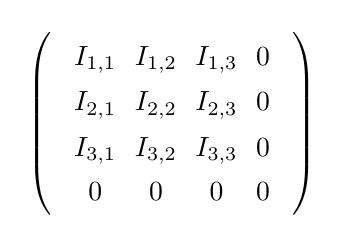
\begin{tikzpicture}[baseline=-\the\dimexpr\fontdimen22\textfont2\relax ]
\matrix (m)[matrix of math nodes,left delimiter=(,right delimiter=)]
{
I_{1,1} & I_{1,2} & I_{1,3} & 0 \\
I_{2,1} & I_{2,2} & I_{2,3} & 0 \\
I_{3,1} & I_{3,2} & I_{3,3} & 0 \\
0       & 0       & 0       & 0 \\
};
\begin{pgfonlayer}{myback}
\fhighlight[green!30]{m-1-1}{m-2-2}
\fhighlight[blue!30]{m-3-3}{m-4-4}
\end{pgfonlayer}
\end{tikzpicture}
\right)
=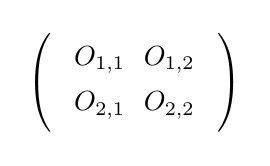
\begin{tikzpicture}[baseline=-\the\dimexpr\fontdimen22\textfont2\relax ]
\matrix (m)[matrix of math nodes,left delimiter=(,right delimiter=)]
{
O_{1,1} & O_{1,2} \\
O_{2,1} & O_{2,2} \\
};
\begin{pgfonlayer}{myback}
\fhighlight[green!30]{m-1-1}{m-1-1}
\fhighlight[blue!30]{m-2-2}{m-2-2}
\end{pgfonlayer}
\end{tikzpicture}
\end{equation}

For example, $O_{1,1} = \max(I_{1,1},I_{1,2},I_{2,1},I_{2,2})$

\subsubsection{Back-propagation}

Here, there is no parameter to adjust, so we just compute the derivative used to continue the back-propagation for each input matrices.
It's similar to the section with the Dense layers and it will be used in the for loop of the back-propagation. We have $O_{a,b}^{(l)} = a_p^{(l)} = a_k^{(l)}$, it's just that we have 2 dimensions instead of one, but if we consider it flatten then it's the same.

\begin{equation}
\begin{split}
    &\forall a,b \in [\![1,w_O]\!]^2, \forall i,j \in [\![(a-1)\times s + 1,a\times s]\!] \times [\![(b-1)\times s + 1,b\times s]\!],\ \frac{\partial O_{a,b}}{\partial I_{i,j}}\\
    &= \begin{cases}
        1 &\text{ if } i,j = \argmax\limits_{k,l \in [\![(a-1)\times s + 1,a\times s]\!] \times [\![(b-1)\times s + 1,b\times s]\!]}(I_{k,l})\\
        0 &\text{ else}
    \end{cases}
\end{split}
\end{equation}

Thus, we have defined above $\frac{\partial z_k^{(l)}}{\partial a_i^{(l-1)}}$ and we have $\frac{\partial a_k^{(l)}}{\partial z_k^{(l)}} = 1$

\newpage
\subsection{Flatten Layer}

This layer take one or multiple input matrices and flatten and concatenate them to get only one vector (dim = 1)

\subsubsection{Feed-forward}

\begin{equation}
flatten(I) = flatten\left(\begin{pmatrix}
I1_{1,1} & I1_{1,2} & I1_{1,3} \\
I1_{2,1} & I1_{2,2} & I1_{2,3} \\
I1_{3,1} & I1_{3,2} & I1_{3,3} \\
\end{pmatrix},\begin{pmatrix}
I2_{1,1} & I2_{1,2} & I2_{1,3} \\
I2_{2,1} & I2_{2,2} & I2_{2,3} \\
I2_{3,1} & I2_{3,2} & I2_{3,3} \\
\end{pmatrix}\right)
=\end{equation}
($I1_{1,1}$, $I1_{1,2}$, $I1_{1,3}$, $I1_{2,1}$, $I1_{2,2}$, $I1_{2,3}$, $I1_{3,1}$, $I1_{3,2}$, $I1_{3,3}$, $I2_{1,1}$, $I2_{1,2}$, $I2_{1,3}$, $I2_{2,1}$, $I2_{2,2}$, $I2_{2,3}$, $I2_{3,1}$, $I2_{3,2}$, $I2_{3,3}$)

\subsubsection{Back-propagation}
There is no derivative involved, we simply revert the flatten transformation, so we need to store the dimensions before the transformation:

($I1_{1,1}$, $I1_{1,2}$, $I1_{1,3}$, $I1_{2,1}$, $I1_{2,2}$, $I1_{2,3}$, $I1_{3,1}$, $I1_{3,2}$, $I1_{3,3}$, $I2_{1,1}$, $I2_{1,2}$, $I2_{1,3}$, $I2_{2,1}$, $I2_{2,2}$, $I2_{2,3}$, $I2_{3,1}$, $I2_{3,2}$, $I2_{3,3}$)
\begin{equation}
\mapsto
\left(\begin{pmatrix}
I1_{1,1} & I1_{1,2} & I1_{1,3} \\
I1_{2,1} & I1_{2,2} & I1_{2,3} \\
I1_{3,1} & I1_{3,2} & I1_{3,3} \\
\end{pmatrix},\begin{pmatrix}
I2_{1,1} & I2_{1,2} & I2_{1,3} \\
I2_{2,1} & I2_{2,2} & I2_{2,3} \\
I2_{3,1} & I2_{3,2} & I2_{3,3} \\
\end{pmatrix}\right)
\end{equation}



\end{document}
